\documentclass[11pt,a4paper]{article}

\usepackage[left=2cm,text={17cm,24cm},top=3cm]{geometry}
\usepackage[slovak]{babel}
\usepackage[utf8]{inputenc}
\usepackage[T1]{fontenc}

\usepackage{url}
\usepackage{tikz}
\usepackage{float}
\usepackage{xcolor}
\usepackage{siunitx}
\usepackage{listings}
\usepackage{csquotes}
\usepackage{hyperref}
\usepackage{textcomp}
\usepackage{breakurl}
\usepackage{etoolbox}
\usepackage{graphicx}
\usepackage{multicol}
\usepackage{multirow}
\usepackage{enumerate}
\usepackage{supertabular}
\usepackage[titles]{tocloft}

\def\UrlBreaks{\do\/\do-}
\newcommand{\red}[1]{\textcolor{red}{#1}}
\newcommand{\TODO}{\textbf{\textcolor{red}{TODO}}}
\newcommand{\tilda}{\raisebox{0.5ex}{\texttildelow}}
\renewcommand{\cftdot}{}

\graphicspath{{img/}}
\setlength\parindent{0pt}
\patchcmd{\thebibliography}{\section*{\refname}}{}{}{}

\begin{document}

\begin{titlepage}
    \begin{center}
        \Huge
        \textsc{
            Fakulta informačních technologií\\
            Vysoké učení technické v~Brně
        }
        \vspace{80px}
        \begin{figure}[!h]
            \centering
            
\includegraphics[scale=0.3]{vutbr-fit-logo.eps}
        \end{figure}
        \\[15mm]
        \Huge{
            \textbf{
                HSC
            }
        }
        \\[1.5mm]
        \huge{
            \textbf{
                Hardware/Software Codesign
            }
        }
        \\[2.5em]
        \LARGE{
            \textbf{
                Vstavaný systém pre filtráciu a segmentáciu obrazu
            }
        }
        \\[2.5em]
        \Large{2018/2019}
        \vfill
    \end{center}
        \Large{
            Adrián Tóth (xtotha01)\hfill \today
        }
\end{titlepage}

\setlength{\parskip}{0pt}
\hypersetup{hidelinks}\tableofcontents
\setlength{\parskip}{0pt}

\newpage
\section{CPU}

Profilovanie CPU časti projektu bolo vykonané pomocou programu \textit{GNU gprof}\footnote{\href{https://sourceware.org/binutils/docs/gprof/}{sourceware.org/binutils/docs/gprof}} verzie \textit{2.26.1}. Desať profilovacích výsledkov bolo nameraných pomocou \textit{návodu z dokumentácie}\footnote{\href{https://sourceware.org/binutils/docs/gprof/Sampling-Error.html}{sourceware.org/binutils/docs/gprof/Sampling-Error.html}} na základe čoho bol vo výsledku jeden sumárny výpis profilovacích hodnôt (priemer desiatich profilovaní).\\

\begin{table}[H]
  \begin{center}
    \begin{tabular}{l|c}
        \multicolumn{1}{c|}{\textbf{Názov}} & \multicolumn{1}{c}{\textbf{Percento času}}\\
        \hline
        \textit{median}            & 62.02 \\
        \textit{gen\_pixel}        & 10.00 \\
        \textit{clip\_window}      & 8.74 \\
        \textit{pixel\_processing} & 5.34 \\
        \textit{shift\_window}     & 4.46 \\
        \textit{buffer}            & 3.66 \\
        \textit{system\_input}     & 2.80 \\
        \textit{thresholding}      & 0.95 \\
        \textit{main}              & 0.79 \\
        \textit{update\_base\_pos} & 0.11 \\
        \textit{histogram\_clean}  & 0.00 \\
        \textit{otsu}              & 0.00 \\
    \end{tabular}
    \caption{Výsledky desiatich profilovaní pomocou \textit{gprof}.}
    \label{tab:gprof}
  \end{center}
\end{table}

\begin{figure}[H]
    \centering
    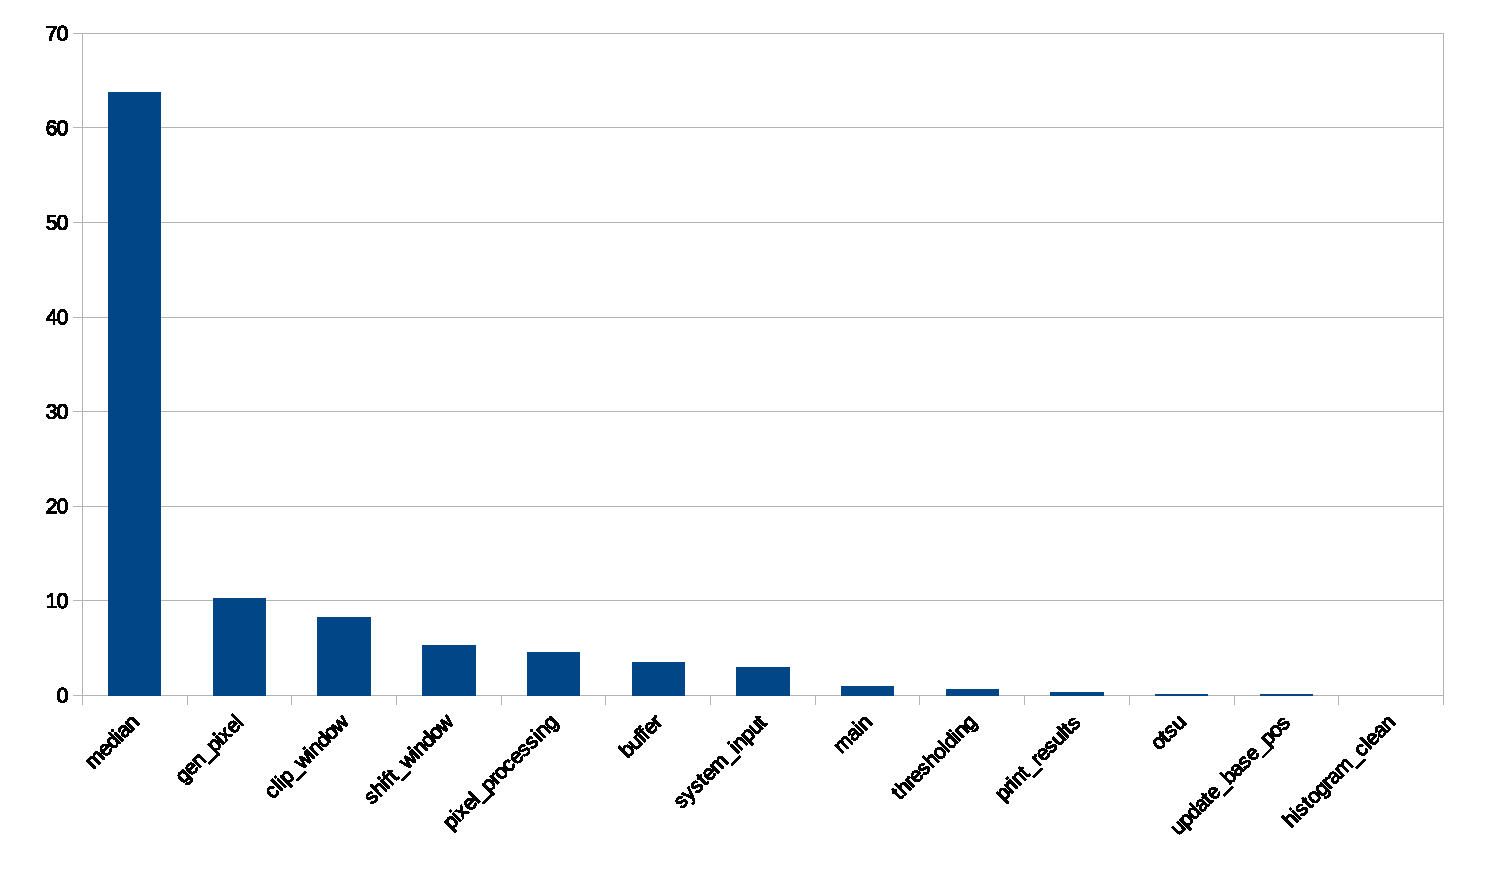
\includegraphics[scale=0.6]{graph.eps}
    \caption{Graf zobrazujúci namerané hodnoty z tabuľky \ref{tab:gprof}.}
    \label{fig:graf}
\end{figure}

\newpage
\section{MCU}

Profilovanie MCU bolo vykonané pomocou makra \texttt{\#define PROFILE}. Výsledky sú zobrazené v tabuľke~\ref{tab:MCU_processing}.

\begin{table}[H]
  \begin{center}
    \begin{tabular}{r|l}
        \multicolumn{1}{c|}{\textbf{Spracovaná časť}} & \multicolumn{1}{c}{\textbf{Čas spracovania}}\\
        \hline
        pixel & $183 \ \mu s$\\
        rámec & $14.0544 \ s$\\
    \end{tabular}
    \caption{Spracovanie určitých častí a ich trvanie na MCU.}
    \label{tab:MCU_processing}
  \end{center}
\end{table}

Implementácia MCU časti je upravená tak aby spracovala 5 rámcov -- rámce číslo 100, 200, 300, 400, 500. Napriek tomu, že sa spracuje len 5 rámcov, doba spracovania piatich rámcov trvá $70.272s$ ($1min \ 10s \ 272ms$). Kebyže implementácia MCU časti nie je upravená -- spracuje sa každý rámec (500 rámcov), tak by spracovanie trvalo $7027.2s$ ($1h \ 57min \ 7s \ 200ms$).

\section{FPGA}

Vlastnosti komponenty pre filtráciu a segmentáciu obrazu:\\[-2em]

\begin{itemize}
    \item V jadre modulu pre \textit{filter} je \textit{main} zreťazený (pipeline enabled) s inicializačným intervalom~4\\[-2em]
    \item Cyklus označený ako \textit{Linit} je rozbalený (unroll enabled)\\[-2em]
    \item Cyklus označený ako \textit{L2} je rozbalený (unroll enabled)\\[-2em]
    \item Cyklus označený ako \textit{L1a} je rozbalený (unroll enabled)\\[-2em]
    \item Cyklus označený ako \textit{L1b} je rozbalený (unroll enabled)\\[-2em]
    \item Latencia obvodu je 4
\end{itemize}

Využitie zdrojov je zobrazené v tabuľke \ref{tab:fpga_resources}.

\begin{table}[H]
  \begin{center}
    \begin{tabular}{l|l}
        Number of Slice Flip Flops & 492 \hspace{1.65mm} out of 1,536 (32\%) \\
        Number of 4 input LUTs     & 1,178 out of 1,536 (76\%) \\
        Number of occupied Slices  & 766 \hspace{1.65mm} out of 768 \hspace{1.65mm} (99\%)   \\
    \end{tabular}
    \caption{Množstvo spotrebovaných zdrojov FPGA čipu.}
    \label{tab:fpga_resources}
  \end{center}
\end{table}

Výpočet času potrebného na spracovanie jednotlivých častí je zobrazený v tabuľke \ref{tab:FPGA_processing}.

\begin{table}[H]
  \begin{center}
    \begin{tabular}{r|l}
        \multicolumn{1}{c|}{\textbf{Spracovaná časť}} & \multicolumn{1}{c}{\textbf{Čas spracovania}}\\
        \hline
        pixel & $160 \ ns$\\
        rámec & $0.012288 \ s$\\
    \end{tabular}
    \caption{Spracovanie určitých častí a ich trvanie na MCU-FPGA.}
    \label{tab:FPGA_processing}
  \end{center}
\end{table}

S rozdelenou implementáciou sa rýchlosť spracovania výrazne zvýšila. Spracovanie všetkých rámcov (500 rámcov) za pomoci rozdelenia SW-HW trvá $6.144s$ ($6s \ 144 ms$).

\section{Porovnanie vlastností SW a SW-HW}\label{sec:comparison}

Časť SW je realizovaná iba na MCU narozdiel od SW-HW ktorá je realizovaná za pomoci MCU a FPGA súčastne. Porovnanie spracovaných častí v SW a SW-HW implementácii je zobrazené v tabuľke~\ref{tab:compare1}.

\begin{table}[H]
  \begin{center}
    \begin{tabular}{r|l|l}
        & \multicolumn{1}{c|}{\textbf{SW}} & \multicolumn{1}{c}{\textbf{SW-HW}}\\
        \hline
        pixel      & $183 \ \mu s$   & $160 \ ns$      \\
        rámec      & $14.0544 \ s$   & $0.012288 \ s$  \\
    \end{tabular}
    \caption{Spracovanie určitých častí a ich trvanie.}
    \label{tab:compare1}
  \end{center}
\end{table}

\hfill\\[-3em]

Rýchlosti spracovania hore uvedených častí (viz tabuľka \ref{tab:compare1}) sú zobrazené v tabuľke~\ref{tab:compare2}.

\begin{table}[H]
  \begin{center}
    \begin{tabular}{r|l|l}
        & \multicolumn{1}{c|}{\textbf{SW}} & \multicolumn{1}{c}{\textbf{SW-HW}}\\
        \hline
        počet pixelov za sekundu & $5464.48087432$ & $6250000$ \\
        počet rámcov za sekundu & $0.07115209471$ & $81.3802083333$ \\
    \end{tabular}
    \caption{Spracovanie určitých častí za jednotku času.}
    \label{tab:compare2}
  \end{center}
\end{table}

\hfill\\[-3em]

Metóda SW-HW implementovaná pomocou MCU-FPGA je o $1143.75$ násobne rýchlejšia od medódy SW ktorá je implementovaná pomocou MCU.

\section{Zhrnutie}

Na základe hore uvedených meraní je zrejmé, že čisto SW a čisto HW realizácia má svoje výhody a nevýhody. Samotná SW realizácia sa ukázala ako značne pomalšia voči ostatným realizáciam. Čisto HW realizácia nie je možná z dôvodu nedostatkov výpočetných zdrojov ktoré sú zreteľne drahšie.\\

Kombináciou SW a HW je ale možné dosiahnuť najefektívnejšiu metódu realizácie, ktorá na základe prepojenia SW a HW umožní realizovať SW pomalé časti v HW ktorý ich vykoná výrazne rýchlejšie.\\

Keďže HW je v našom prípade limitovaný v rámci zdrojov, treba zvážiť na základe rýchlosti ktoré časti (časti ktoré sú v SW značne pomalé) treba previesť do HW keďže nie všetky je možné previesť. V našom prípade bola najpomalšia časť SW funkcia \textit{median} ale keďže bolo dostatok zdrojov ešte aj na ďalšie funkcie previedli sa aj ďalšie pomalé funkcie. Pri správnom rozdelení a prevode je výsledná realizácia výrazne rýchlejšia -- v našom prípade až $1143.75$ krát rýchlejšia.\\

Ak by HW (čip FPGA) obsahoval dostatok zdrojov na to aby bolo možné presunúť zvyšné SW časti do HW (realizácia čisto v HW), zrýchlenie by bolo najväčšie. Problémom ale je, že v HW je výpočetná kapacita výrazne limitovaná cenou.

%\newpage
%\section{Literatúra}
%\bibliographystyle{slovakiso}
%\begin{flushleft}
%    \bibliography{quotation}
%\end{flushleft}

\end{document}
